\section{Implementation}
\subsection{Clients}
The three main components are implemented with the low level Java client APIs of the platforms. Consumer clients of the platforms are used to subscribe and read messages on the streams while producer clients are used to publish messages to the platforms.

\textbf{Event generator and Stream processor}
\begin{figure}[h!]
	\centering
	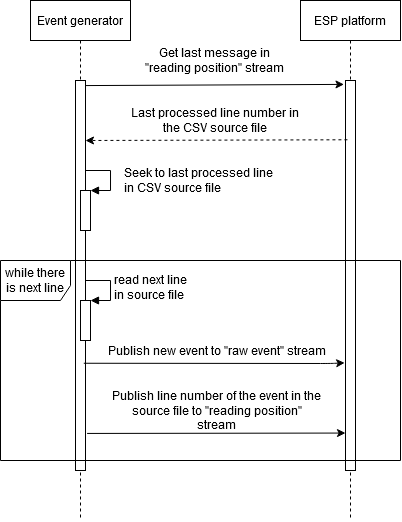
\includegraphics[width=11cm]{images/implement-event-generator.png}
	\caption{Sequence diagram of event generator component.}
	\label{fig:implementeventgenerator}
\end{figure}


\begin{figure}[h!]
	\centering
	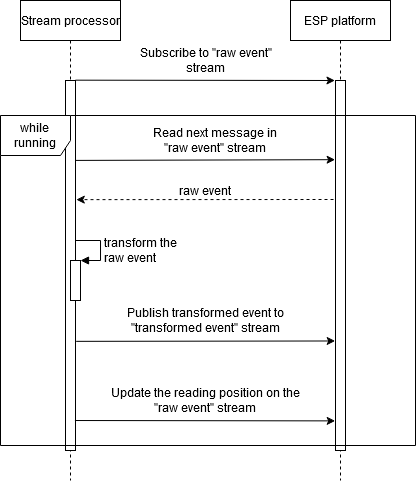
\includegraphics[width=11cm]{images/implement-stream-processor.png}
	\caption{Sequence diagram of stream processor component.}
	\label{fig:implementstreamprocessor}
\end{figure}
\iffalse
\begin{figure}[ht!]
	\begin{adjustwidth}{-1cm}{-1cm}
	\centering
	\begin{minipage}[t]{.48\linewidth}
		\centering
		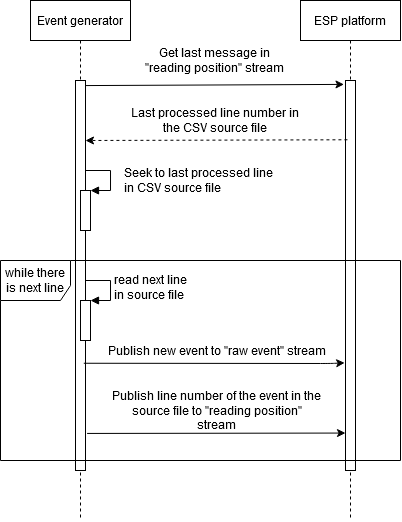
\includegraphics[width=\linewidth]{images/implement-event-generator.png}
		\caption{Sequence diagram of event generator component.}
		\label{fig:implementeventgenerator1}
	\end{minipage}%
	\hfill
	\begin{minipage}[t]{.48\linewidth}
		\centering
		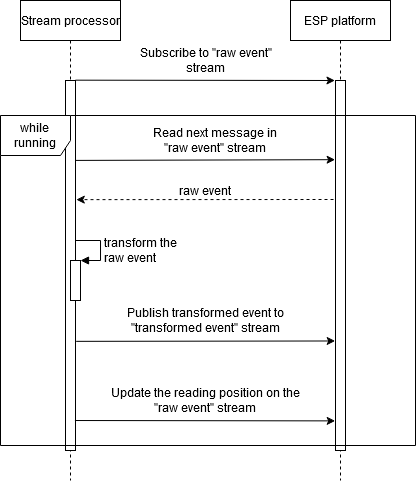
\includegraphics[width=\linewidth]{images/implement-stream-processor.png}
		\caption{Sequence diagram of stream processor component.}
		\label{fig:implementstreamprocessor1}
	\end{minipage}
	\end{adjustwidth}
\end{figure}
\fi
Figures \ref{fig:implementeventgenerator} and \ref{fig:implementstreamprocessor} show the sequence diagrams of the event generator and the stream processor respectively. With Apache Kafka and Apache Pulsar, to achieve exactly-once semantics with these two components,  the two operations to publish events and update the reading position on the data source must be atomically combined with the transaction features of the two platforms. 

Listing \ref{lst:kafkastreamprocessor} shows part of the source code of the stream processor component for Kafka. The transaction, in which transformed events are published to \emph{transformed-event} topic and the offset numbers of consumed messages on \emph{raw-event} topic are committed to Kafka, is started on line 12 and committed on line 29. 
\newpage

\lstinputlisting[label={lst:kafkastreamprocessor},language=Java,caption={Kafka stream processor with the transaction feature.}]{chapters/implementation/KafkaStreamProcessor.java} 

To ensure exactly-once semantics, Kafka has fencing mechanism in its transactions to prevent duplication of messages and notify users by throwing back exceptions. When there is two producer instances with the same ID trying to publish messages to Kafka, requests from older instance will be rejected by Kafka and a \emph{ProducerFencedException} will be returned to this instance. When a temporarily disconnected application is replaced by a newer instance and the old instance later reconnects, this could lead to two instances sending the same message simultaneously. This fencing mechanism helps prevent that scenario. 

Fencing mechanism of Kafka also prevents messages duplication when partition reassignment occurs within a consumer group \cite{kafkatransctionscaleproducer}. When the offset number of source topic is committed in a transaction (as in line 25 in listing \ref{lst:kafkastreamprocessor}), the metadata of the consumer which is used to read the input message must also be sent to Kafka. When this offset committing request is accepted by Kafka, the partition to which the message belongs is locked by the consumer instance declared in the request. If partition reassignment is triggered after the lock is obtained, the new owner of the reassigned partition must wait until the ongoing transaction on the locked partition is either completed, aborted or timeout before it can pull new messages from Kafka. Moreover, Kafka ensures that a partition can only be locked by a consumer with up-to-date metadata. When a consumer is unaware of the latest partition reassignment, its metadata becomes obsolete and any offset committing requests with this consumer will be rejected by Kafka and a \emph{CommitFailedException} will be returned. Any stream processor instance with the consumer whose metadata is not up-to-date cannot publish any new message. In this case, the transaction should simply be aborted and latest metadata of the consumer group about partitions assignment must be retrieved from Kafka.

The implementation of the event generator with Kafka transaction is fairly similar. However, since the event generator reads input data from the CSV file rather than a Kafka topic, it only publishes reading position as a normal message to Kafka in the same transaction instead of committing offset number as in the stream processor.

For Apache Pulsar, listing \ref{lst:pulsarstreamprocessor} shows part of the source code for the stream processor with the transaction feature. 

\lstinputlisting[label={lst:pulsarstreamprocessor},language=Java,caption={Pulsar stream processor with the transaction feature.}]{chapters/implementation/PulsarStreamProcessor.java} 

In the transaction from line 15 to line 30, the transformed event and the acknowledgement of the corresponding raw event are sent to Pulsar as an atomic operation. Pulsar handles the case of partition reassignment within a consumer group quite differently from Kafka to ensure exactly-once semantics. When a consumer acknowledge the consumption of a message in a transaction (line 29 in listing \ref{lst:pulsarstreamprocessor}), Pulsar locks this message for that specific consumer \cite{pulsartransaction} until the transaction is completed or aborted. If a message on a partition is locked before partition reassignment occurs, it will not be redelivered to the new owner of the partition. On the other hand, if rebalancing happens before an application instance acknowledges and obtains lock on a message, this message will be redelivered to the new owner of the partition and therefore simultaneously exists on the buffers of two different consumer instances. In this case, the first application instance to finish processing and acknowledge will obtain the lock and cause the other instance to back off with a \emph{TransactionConflictException} when it tries to acknowledge the same message.

The transaction in Pulsar event generator is implemented similarly. Instead of acknowledging message on the source topic, the event generator update the reading position by publishing the line number of published event in the CSV file in the same transaction. 

With NATS Streaming, atomically publishing and acknowledging the consumption of multiple messages is not supported. Therefore, the event generator and stream processor are implemented according to the sequence diagrams in figures \ref{fig:implementeventgenerator} and \ref{fig:implementstreamprocessor} without any special remark.

\textbf{View generator}

Regarding the view generator component, the implementations on all three platforms are fairly similar. To interact with the relational database and map Java object to relational table, the OpenJPA which is an implementation of Java Persistence API (JPA) \cite{jpa} is used. Two entities, namely, \emph{CurrentBalance} and \emph{CurrentReadingPosition} (listings \ref{lst:currentbalance} and \ref{lst:currentreadingposition}), representing the snapshot of current balances and reading position on the source stream respectively are defined and mapped to two corresponding tables on the PostgreSQL database.   
\newpage

\lstinputlisting[label={lst:currentbalance},language=Java,caption={Current balance entity.}]{chapters/implementation/CurrentBalance.java} 

In the current balance entity, apart from the customer ID and the current balance of the corresponding customer, there is an additional field which indicates the source partition to which events from this customer is published on the ESP platform. This field is applicable in case of Kafka and Pulsar where multiple view generator instances can consume the \emph{transformed-event} topic concurrently. When an application instance is assigned a partition, it must use this source partition field to retrieve the latest snapshots of current balances of all customers on this partition. In case of NATS Streaming, topic cannot be partitioned and therefore this field will simply be assigned a default value. 


\lstinputlisting[label={lst:currentreadingposition},language=Java,caption={Current reading position entity.}]{chapters/implementation/CurrentReadingPosition.java} 
For the current reading position entity, each partition on the source topic will be mapped to a row in the database table and is uniquely identified by the partition number. In case of NATS Streaming, there is only one row with the default partition number. 


Figure \ref{fig:implementviewgenerator} illustrates the overall workflow of the view generator component.
\newpage
\begin{figure}[h]
	\centering
	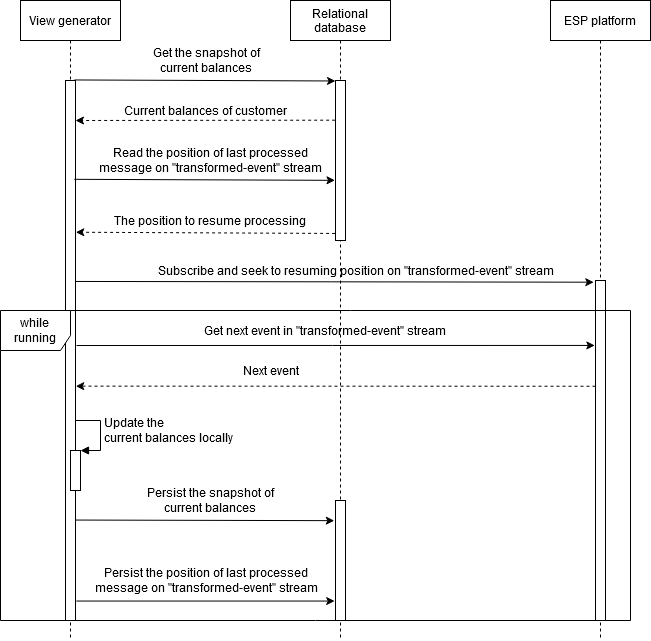
\includegraphics[width=\linewidth]{images/implement-view-generator.png}
	\caption{Sequence diagram of view generator component.}
	\label{fig:implementviewgenerator}
\end{figure}

The two operations to persist snapshot of current balances and corresponding reading position are conducted in a transaction to ensure the atomicity and guarantee exactly-once semantics in case the view generator crashes in the middle on a transaction.

\subsection{Failure injection}
To provoke failure scenarios described in section \ref{subsection:failurescenarios}, custom codes are injected into the the application at runtime to pause or terminate the program using Byteman tracing tool for Java \cite{byteman}. With this tool, Byteman rule can be defined to inject arbitrary code into a running application when a condition is met. A Byteman rule contains of three main parts: 
\begin{itemize}
	\item Event: this triggers the rule
	\item Condition: this part checks the current status of the running application
	\item Action: this part defines the alternative behavior of the application if the condition is satisfied
\end{itemize}


\lstinputlisting[label={lst:bytemanrule},language=Java,caption={Byteman rule script for stream-processor-crash scenario on Kafka.}]{chapters/implementation/byteman.btm} 

In the example in listing \ref{lst:bytemanrule} is the Byteman rule to inject failure during runtime into the stream processor component of Kafka. The event is defined from line 2 to 4. When the method \emph{bytemanHook} in the class \emph{KafkaStreamProcessor} is executed, the rule is invoked. The \emph{bytemanHook} is a predefined helper method to provide a convenient way to specify the injecting position in the class without having to modify much in the application code. In the stream processor class of Kafka (listing \ref{lst:kafkastreamprocessor}), this method is placed between the operations to publish transformed events and commit offset of processed raw events. The \emph{bytemanHook} method does nothing and accepts as parameter a counter variable indicating the number of messages which have been processed by the processor since started. This counter is used in the condition of the Byteman rules online 6, namely, when the stream processor has processed and published successfully more than 120 messages, the action defined on line 7 which intentionally terminates the application is executed.

Different rules corresponding to different failure scenarios on each processing components are defined similarly for all three platforms. To execute the application with defined Byteman rule, the Java virtual machine (JVM) must be configured to load and run the executable jar file of the Byteman engine when the application is executed. In addition, the script of the rule to be executed must be specified as well.

\lstinputlisting[label={lst:bytemanruleexecute},keywordstyle={\color{blue}},language=bash,caption={Execute the stream processor of Kafka with the Byteman rule.}]{chapters/implementation/byteman.sh} 

\subsection{Running environment}
To run the failure scenarios on each platform, Docker compose is used to containerize required infrastructure and processing components and run them locally in a Docker environment \cite{docker}.

The infrastructure comprises of the ESP platform and the PostgreSQL relational database. The ESP platforms are set up with multiple instances running in different Docker containers to be fault-tolerant:
\begin{itemize}
	\item Apache Kafka: three Zookeeper instances and three Kafka broker instances.
	\item Apache Pulsar: three Zookeeper instances, three BookKeeper instances and two Pulsar broker instances.
	\item NATS Streaming: three NATS Streaming server instances in clustering mode and file-based persistence.
\end{itemize}

While Apache Pulsar and NATS Streaming have official Docker images, Apache Kafka is not released with a Docker image. Nevertheless, there are a number of Kafka Docker images provided by third-party organizations. In the thesis, the Kafka Docker image from the company Confluent is used as it is regularly updated.

Regarding the processing components, their executable files are containerized and run in the same Docker environment as the infrastructure. For each processing component, different containers are prepared for the normal instance without failure and the fault-injected instance by Byteman. 

To conveniently start the failure scenarios, scripts are prepared to start up the Docker containers of the infrastructure, create the necessary streams on the platforms, and run the processing components.
 